\documentclass[oneside,final,12pt]{article}
\usepackage[utf8x]{inputenc}
\usepackage[english, russian]{babel}
\usepackage{vmargin}
\usepackage{amsfonts}
\usepackage[T1]{fontenc}
\usepackage{graphicx}
\usepackage{csvsimple}
\usepackage{tikz}
\usepackage{cmap}
\setlength{\parindent}{5ex}
\graphicspath{{pictures3/}}
\DeclareGraphicsExtensions{.pdf,.png,.jpg}
\setpapersize{A4}
\setmarginsrb{2cm}{1.5cm}{1cm}{1.5cm}{0pt}{0mm}{0pt}{13mm}
\usepackage{indentfirst}
\usepackage{tikz}
\usepackage{hyperref}
\hypersetup{
    colorlinks=true,
    linkcolor=blue,
    filecolor=magenta,      
    urlcolor=cyan,
    pdftitle={Overleaf Example},
    pdfpagemode=FullScreen,
    }
\sloppy

\begin{document}
Бычков Георгий 317
\tableofcontents
\newpage

\section {Введение}
	В данном отчете изучаются алгоритмы случайный лес и градиентный бустинг. В качестве источника данных, на которых проводится исследование, было выбрано соревнование House Sales in King County, USA по \href{https://www.kaggle.com/harlfoxem/housesalesprediction}{адресу}.

\section {Обработка данных}
	Для удобства работы с представленными данными нужно перевести их в числовой формат. Анализ столбцов исходной матрицы данных показал, что почти все столбцы имеют целый или вещественный тип, за исключением столбца с датой. Было решено столбец с датой превратить в 3 столбца с годом, месяцем и номером дня в месяце. Это расширит признаковое пространство и можно будет создавать большее число комбинаций признаков в деревьях . В итоге у нас получается матрица из вещественных чисел, которую можно перевести в массив numpy.

\section {Исследование случайного леса}
	В данной части будет рассмотрен алгоритм случайного леса на приведенном наборе данных. Будет исследованы его результаты при разных значениях входных гиперпараметров.
\begin{figure}[h!]
\center{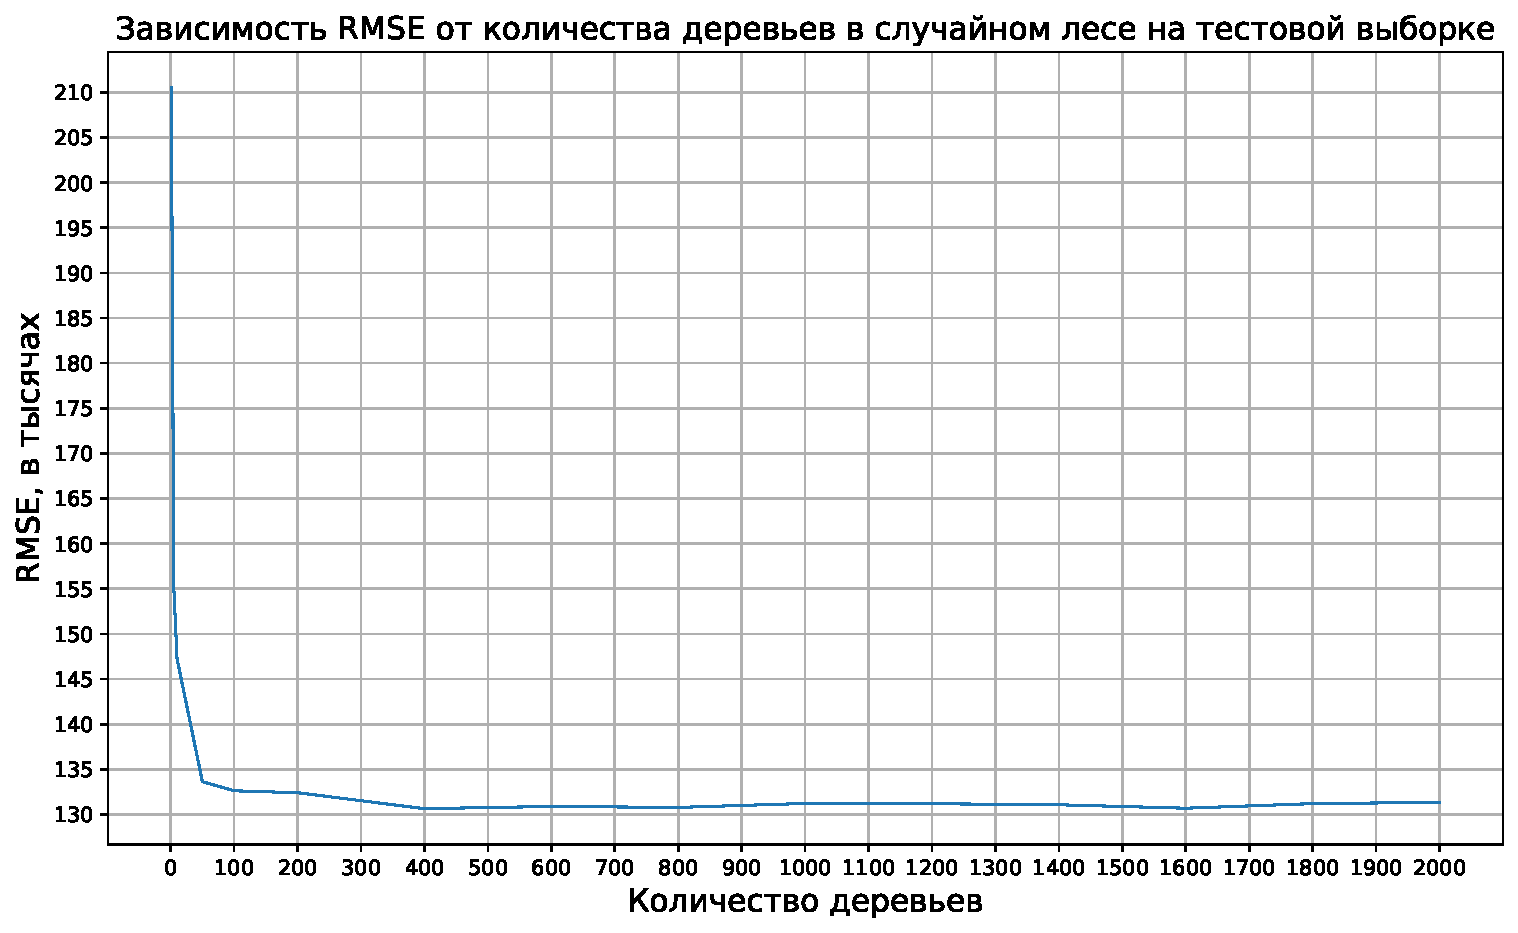
\includegraphics[scale=0.55]{1.1}}
\caption{Зависимость функции потерь (RMSE) от количества деревьев}
\label{fig:image1}
\end{figure}
\subsection {Подбор оптимального количества деревьев}
	Первым параметром подбирается количество деревьев в алгоритме. Остальные параметры задаются по умолчанию. Как видно из графика, с ростом количества деревьев, точность алгоритма сначала увеличивается, но начиная с некоторого значения, увеличение количества деревьев не приводит к изменению функциии ошибок. 

Что касается времени выполнения программы, то оно зависит линейно от количества деревьев, как можно видеть на графике. Оптимальным значением можно взять 600 деревьев, так как при этом времени программа будет работать быстрее всего, не теряя точности.
\begin{figure}[h!]
\center{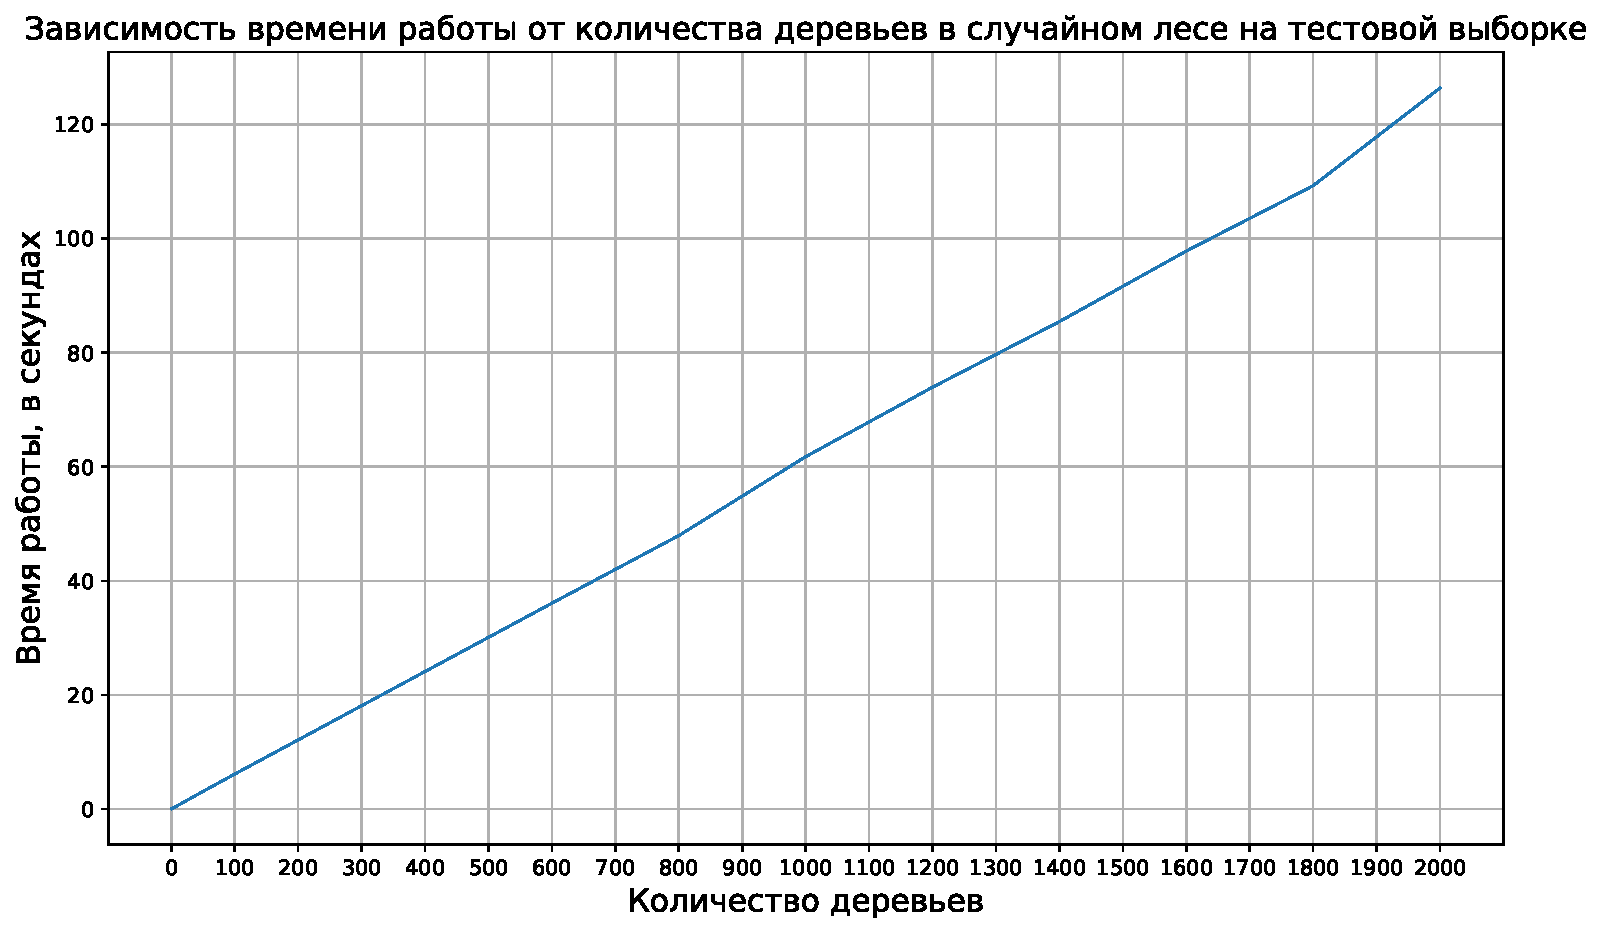
\includegraphics[scale=0.55]{1.2}}
\caption{Зависимость времени выполнения программы от количества деревьев}
\label{fig:image2}
\end{figure}
\begin{figure}[h!]
\center{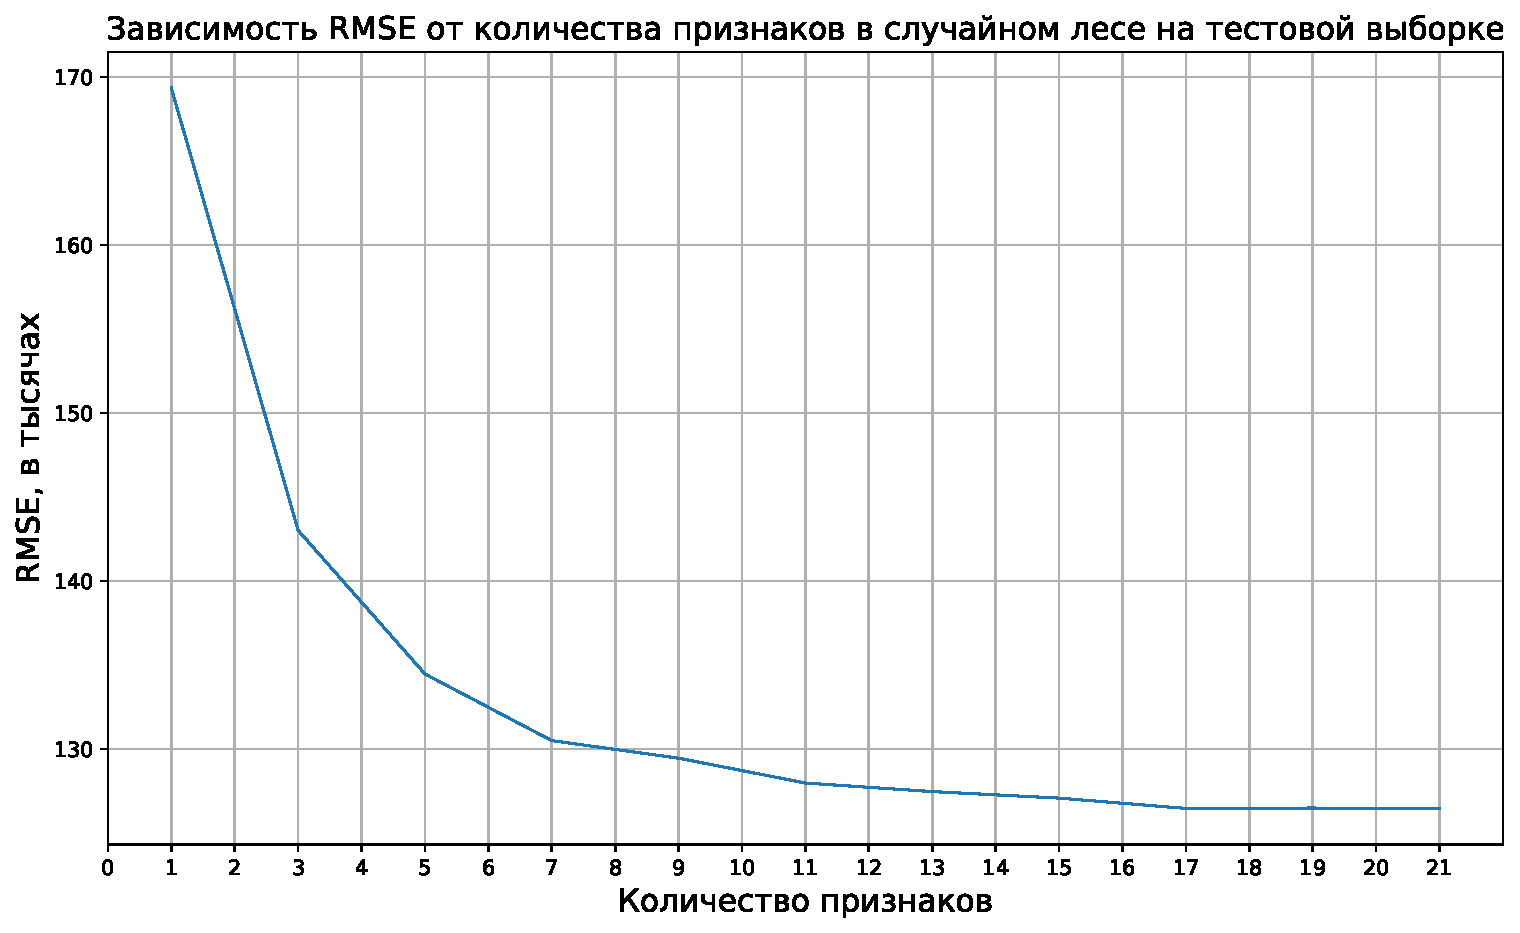
\includegraphics[scale=0.55]{2.1}}
\caption{Зависимость функции потерь (RMSE) от количества признаков}
\label{fig:image3}
\end{figure}
\subsection {Подбор оптимального количества признаков}
	Затем подбирается оптимальное количество признаков. Количество деревьев равно 600, остальные параметры берутся по умолчанию. Как видно из графика, с ростом количества признаков значение RMSE убывает и начиная с некоторого значения точность остается почти неизменной. 

С ростом числа признаков, время работы алгоритма растет линейно. Поэтому можно считать оптимальным количество признаков равным 17, так как это наименьшее значение, при котором качество остается на почти минимальном уровне, то есть алгоритм будет работать наиболее быстро с той же точностью.
\begin{figure}[h!]
\center{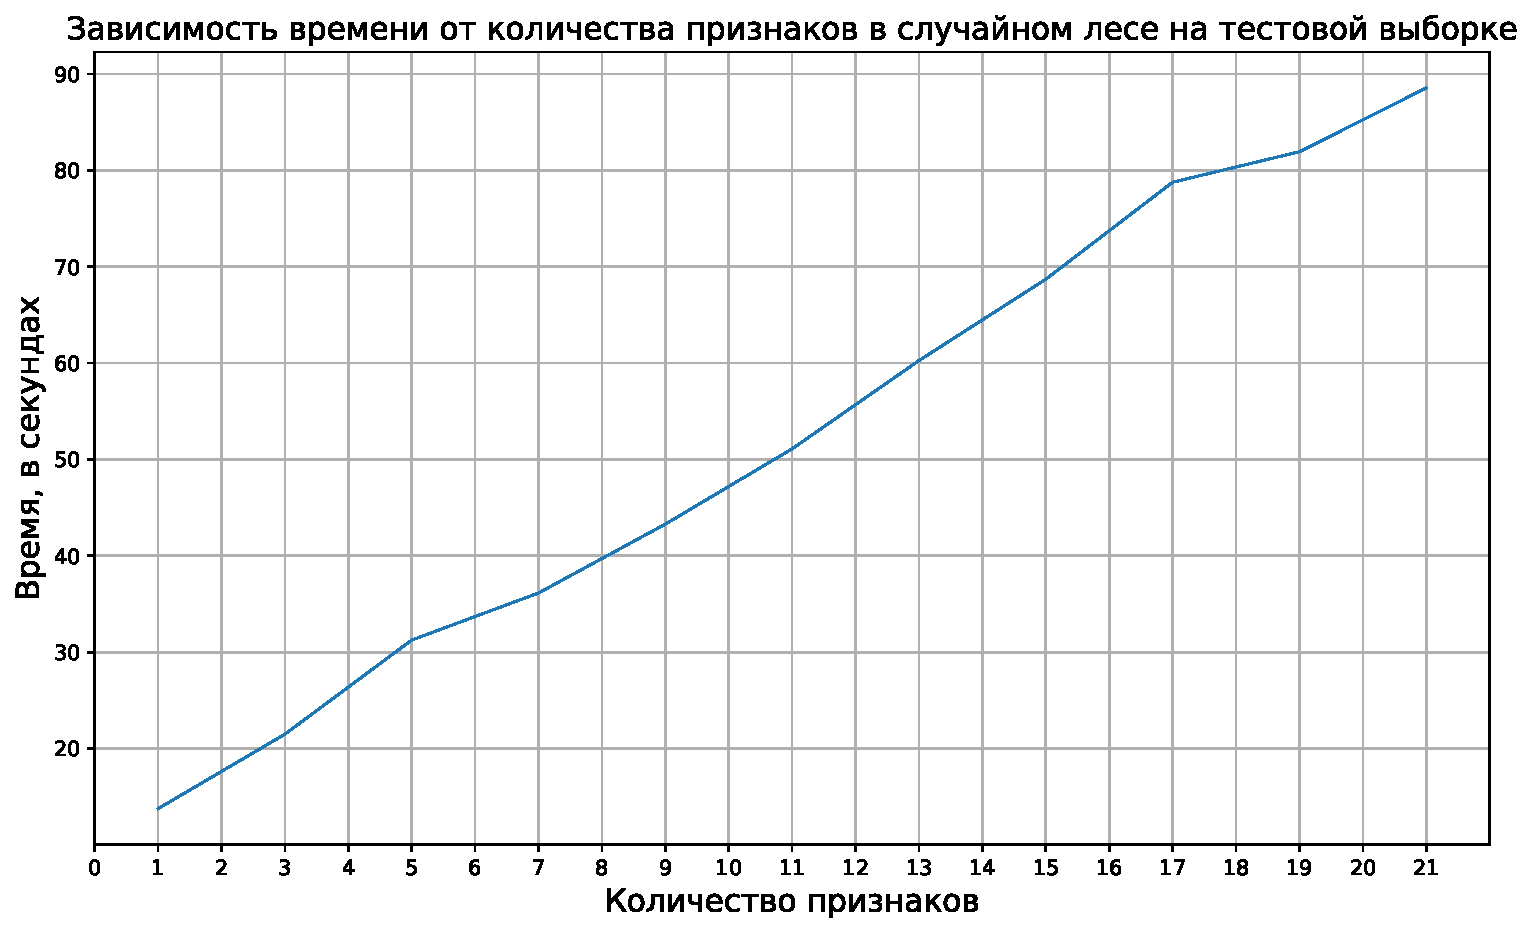
\includegraphics[scale=0.55]{2.2}}
\caption{Зависимость времени выполнения программы от количества признаков}
\label{fig:image4}
\end{figure}
\begin{figure}[h!]
\center{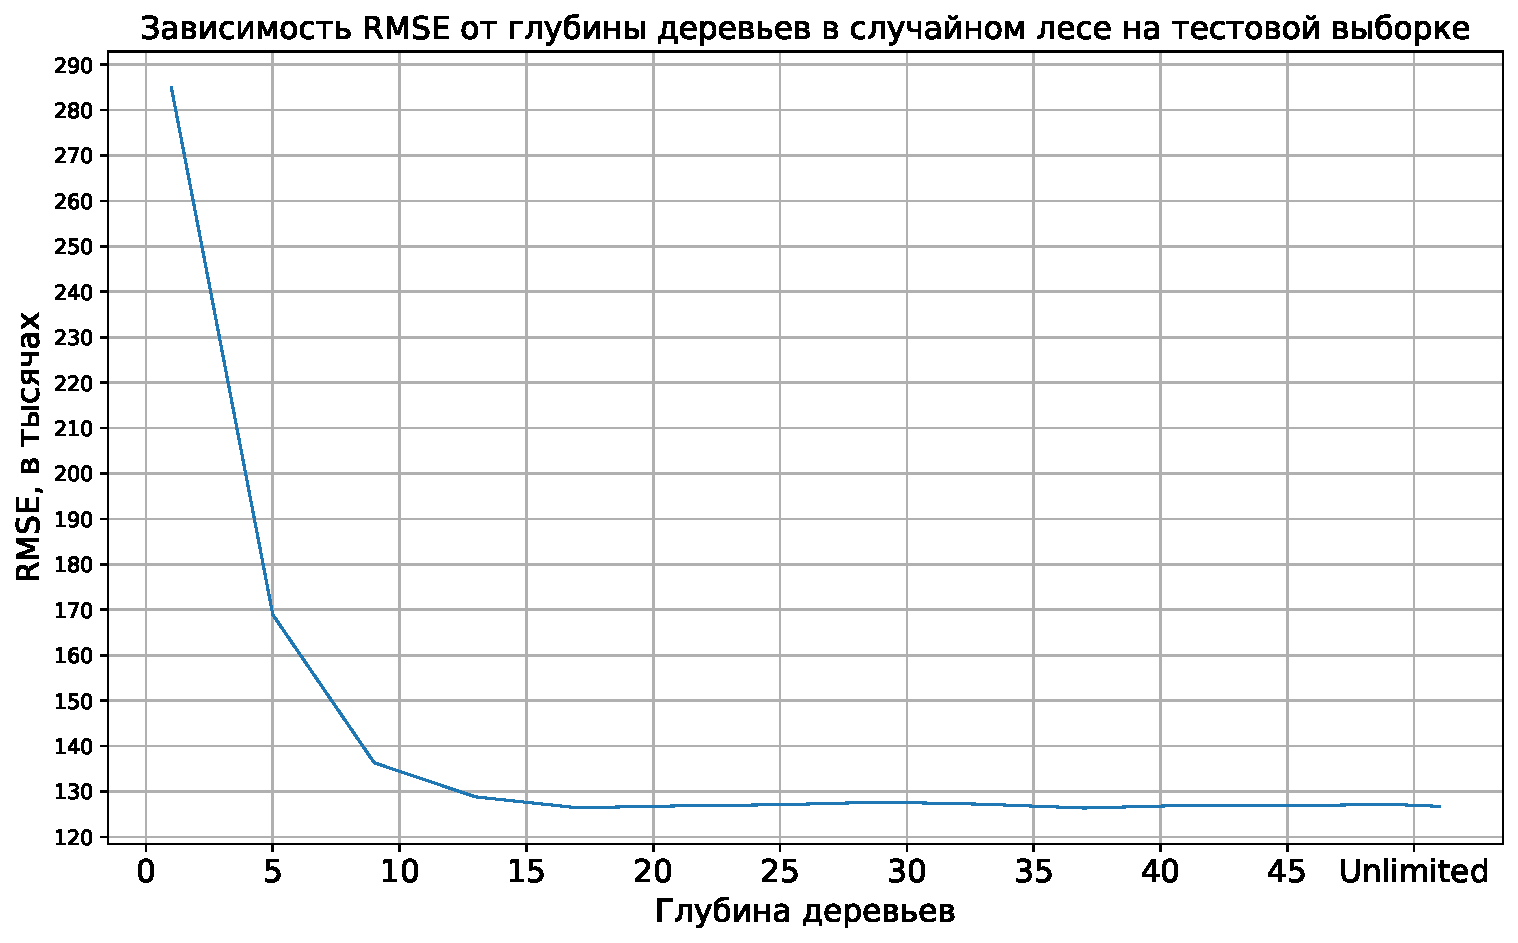
\includegraphics[scale=0.55]{3.1}}
\caption{Зависимость функции потерь (RMSE) от максимальной глубины деревьев}
\label{fig:image5}
\end{figure}
\subsection {Подбор оптимальной глубины деревьев}
	Следующим подбирается оптимальное значение глубины деревьев. Были рассмотрены значения максимальной глубины до 50, а также отдельно случай с неограниченным деревом. Как видно из графика, более глубокие (переобученные) деревья будут давать лучшую точность на тестовой выборке.

Время обучения в этот раз зависит линейно от параметра только при глубине меньшей 15, затем она начинает выходить на практически постоянное значение. Таким образом, лучшую точность будут давать глубокие деревья.
\begin{figure}[h!]
\center{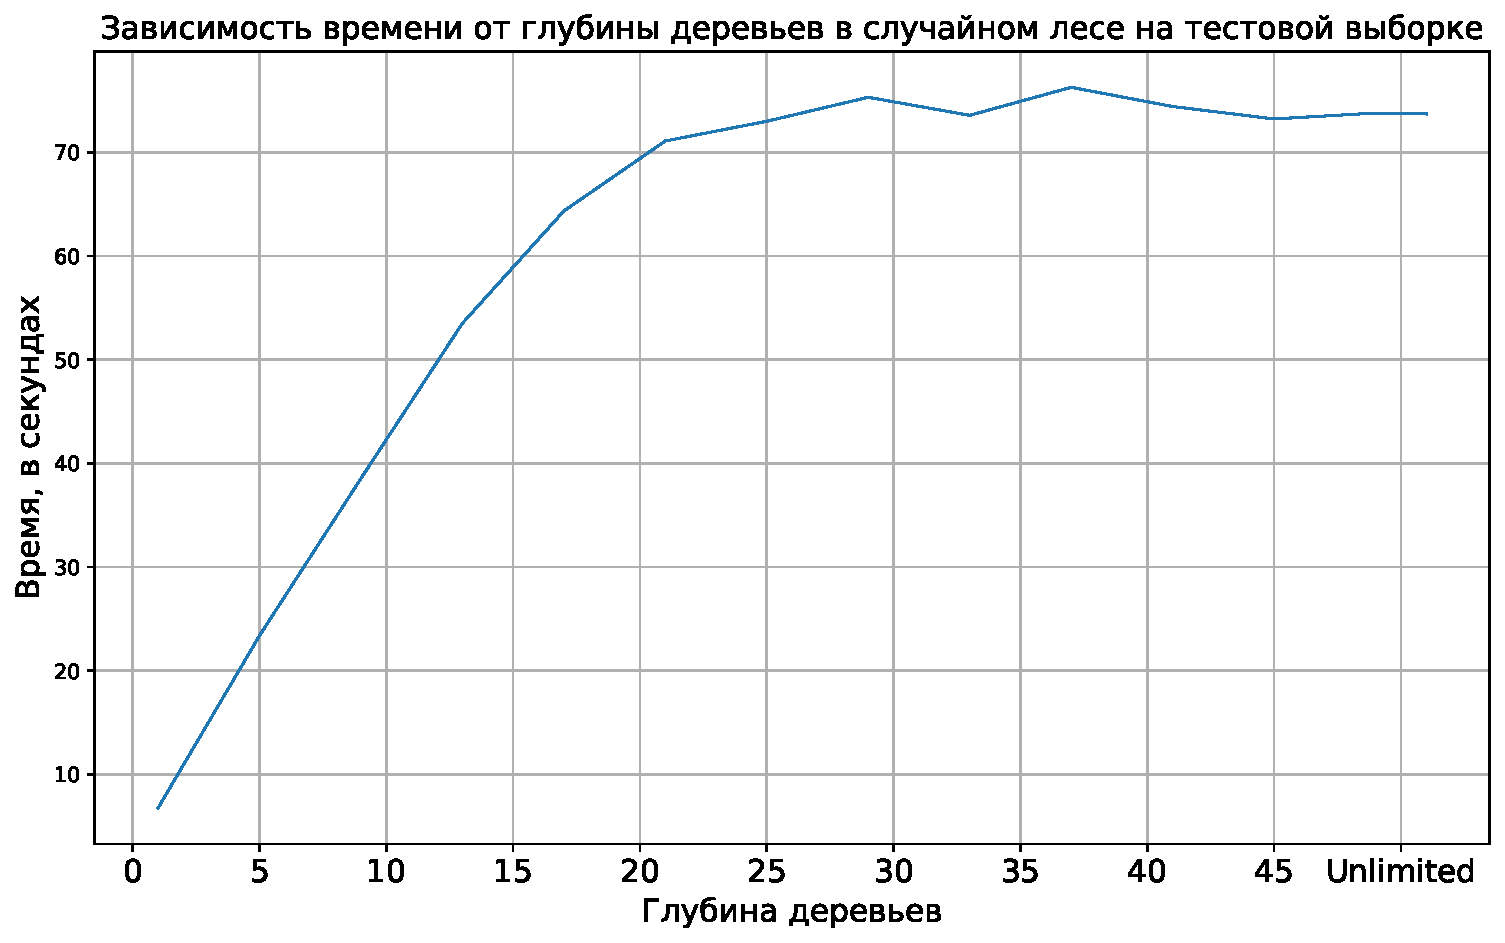
\includegraphics[scale=0.55]{3.2}}
\caption{Зависимость времени выполнения программы от максимальной глубины деревьев}
\label{fig:image6}
\end{figure}
\section {Исследование градиентного бустинга}
	В данной части будет исследован градиентный бустинг над деревьями и его значения в зависимости от следующих гиперпараметров: количество деревьев, максимальное количество признаков, максимальная глубина, скорость обучения.
\begin{figure}[h!]
\center{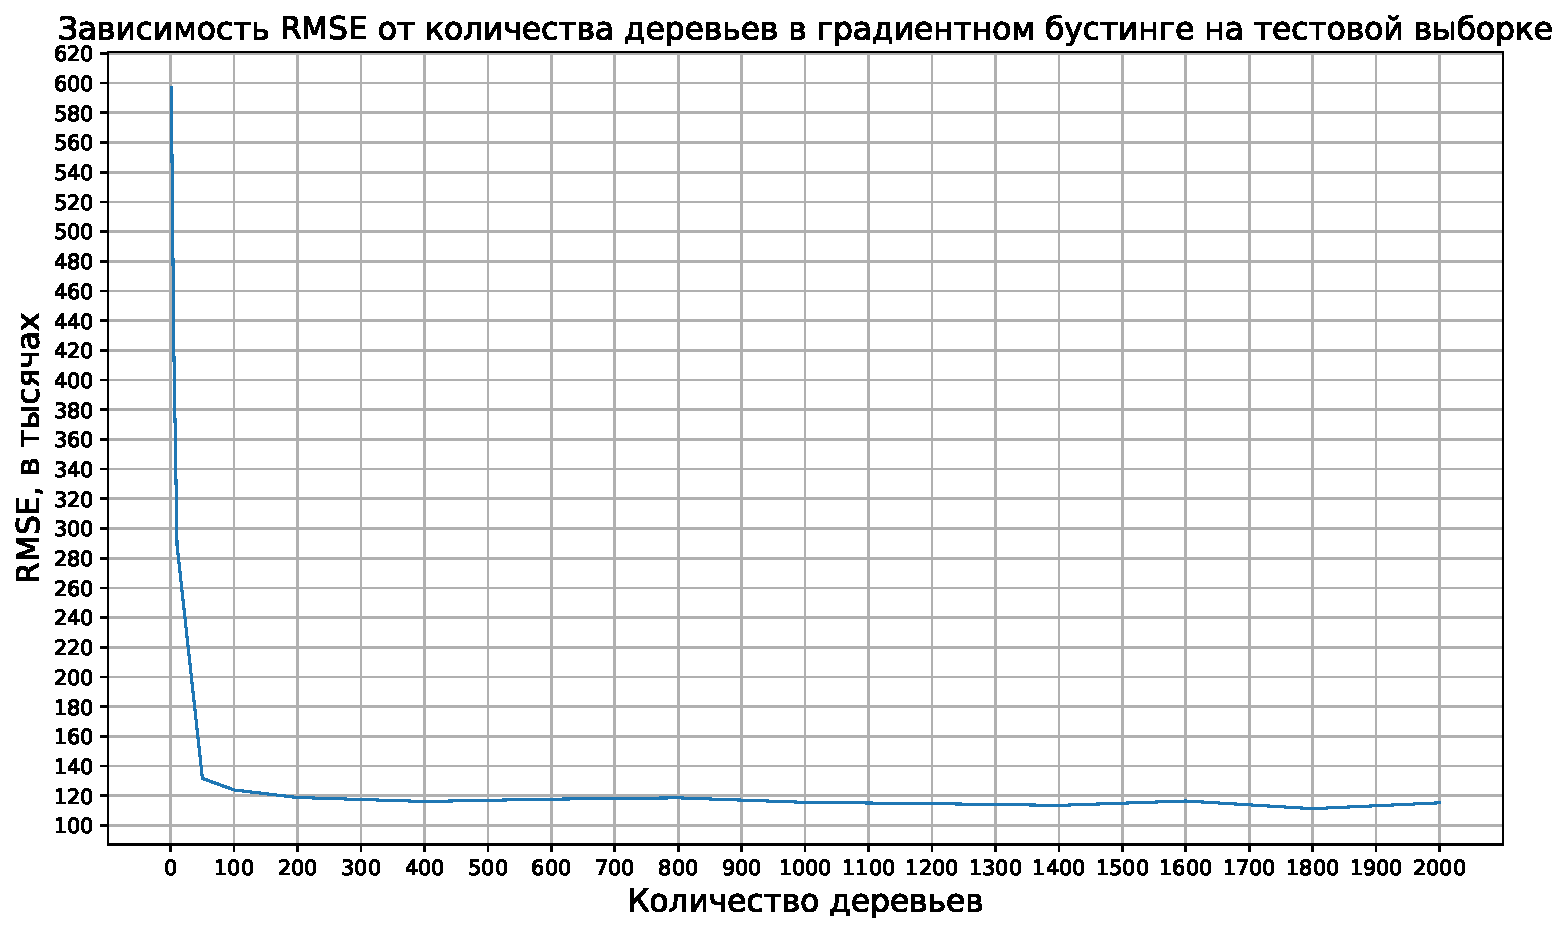
\includegraphics[scale=0.55]{4.1}}
\caption{Зависимость функции потерь (RMSE) от количества деревьев}
\label{fig:image7}
\end{figure}
\subsection {Подбор оптимального количества деревьев}
	Первым параметром подбирается количество деревьев в алгоритме. Остальные параметры задаются по умолчанию, темп обучения по умолчанию принят равным 0.1. Как видно из графика, с ростом количества деревьев растет его точность и, как и в случае с случайным лесом, начиная с некоторого количества деревьев, точность не будет сильно меняться.

	От количества деревьев время работы программы зависит так же линейно. Можно принять оптимальным значение в 1000 деревьев по таким же соображениям: наименее затратное по времени, с высокой точностью.

\begin{figure}[h!]
\center{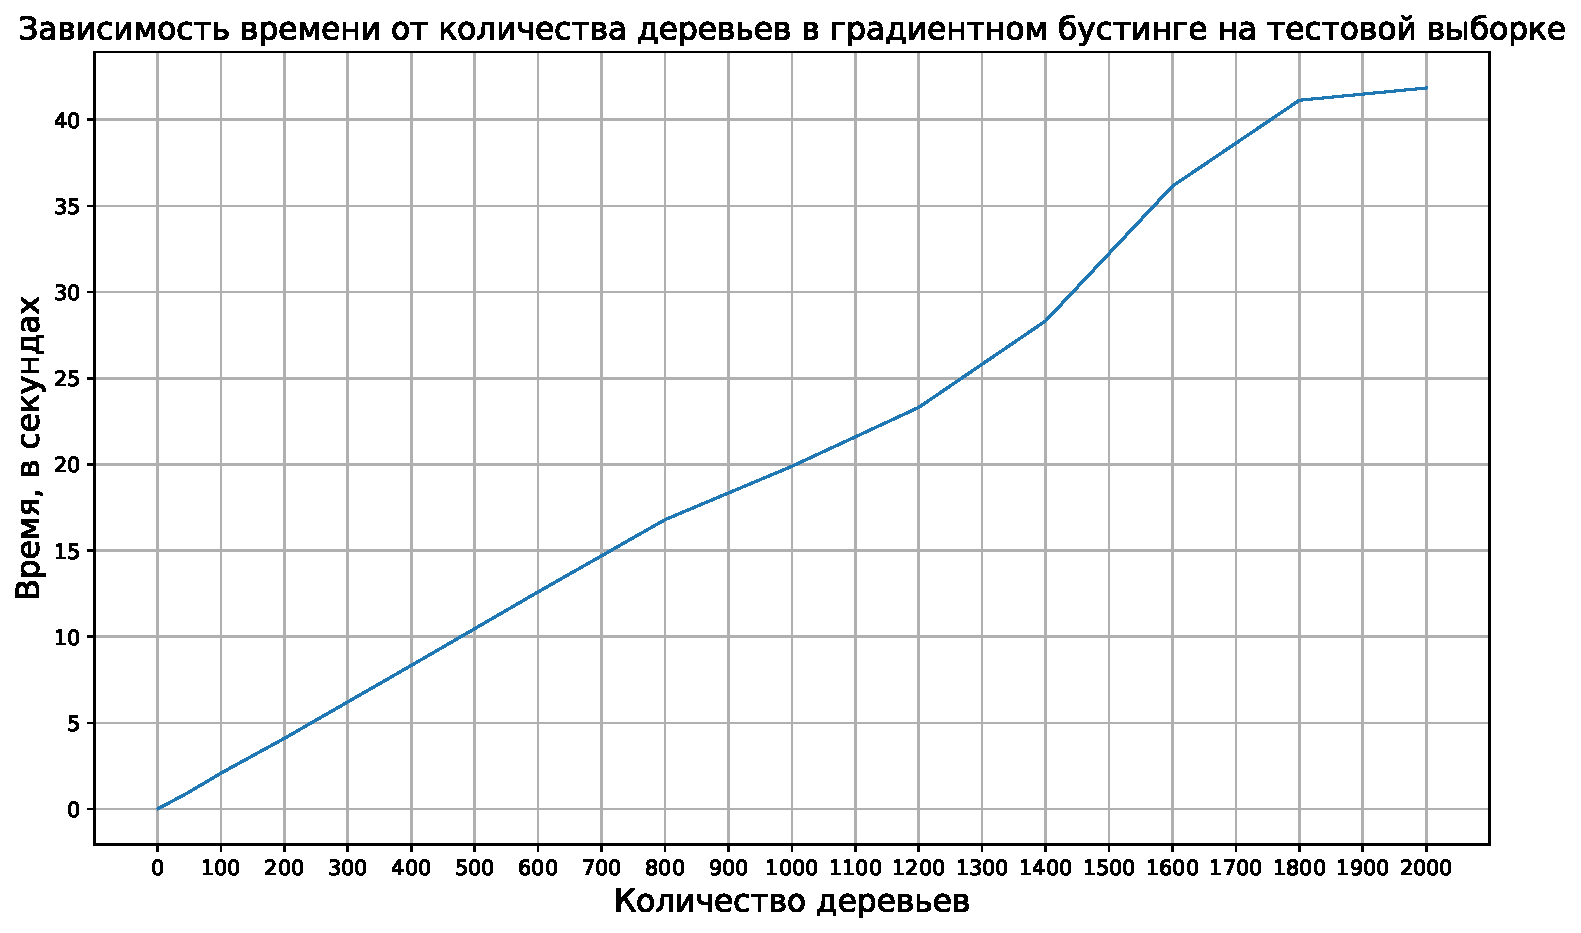
\includegraphics[scale=0.55]{4.2}}
\caption{Зависимость времени выполнения программы от количества деревьев}
\label{fig:image8}
\end{figure}
\begin{figure}[h!]
\center{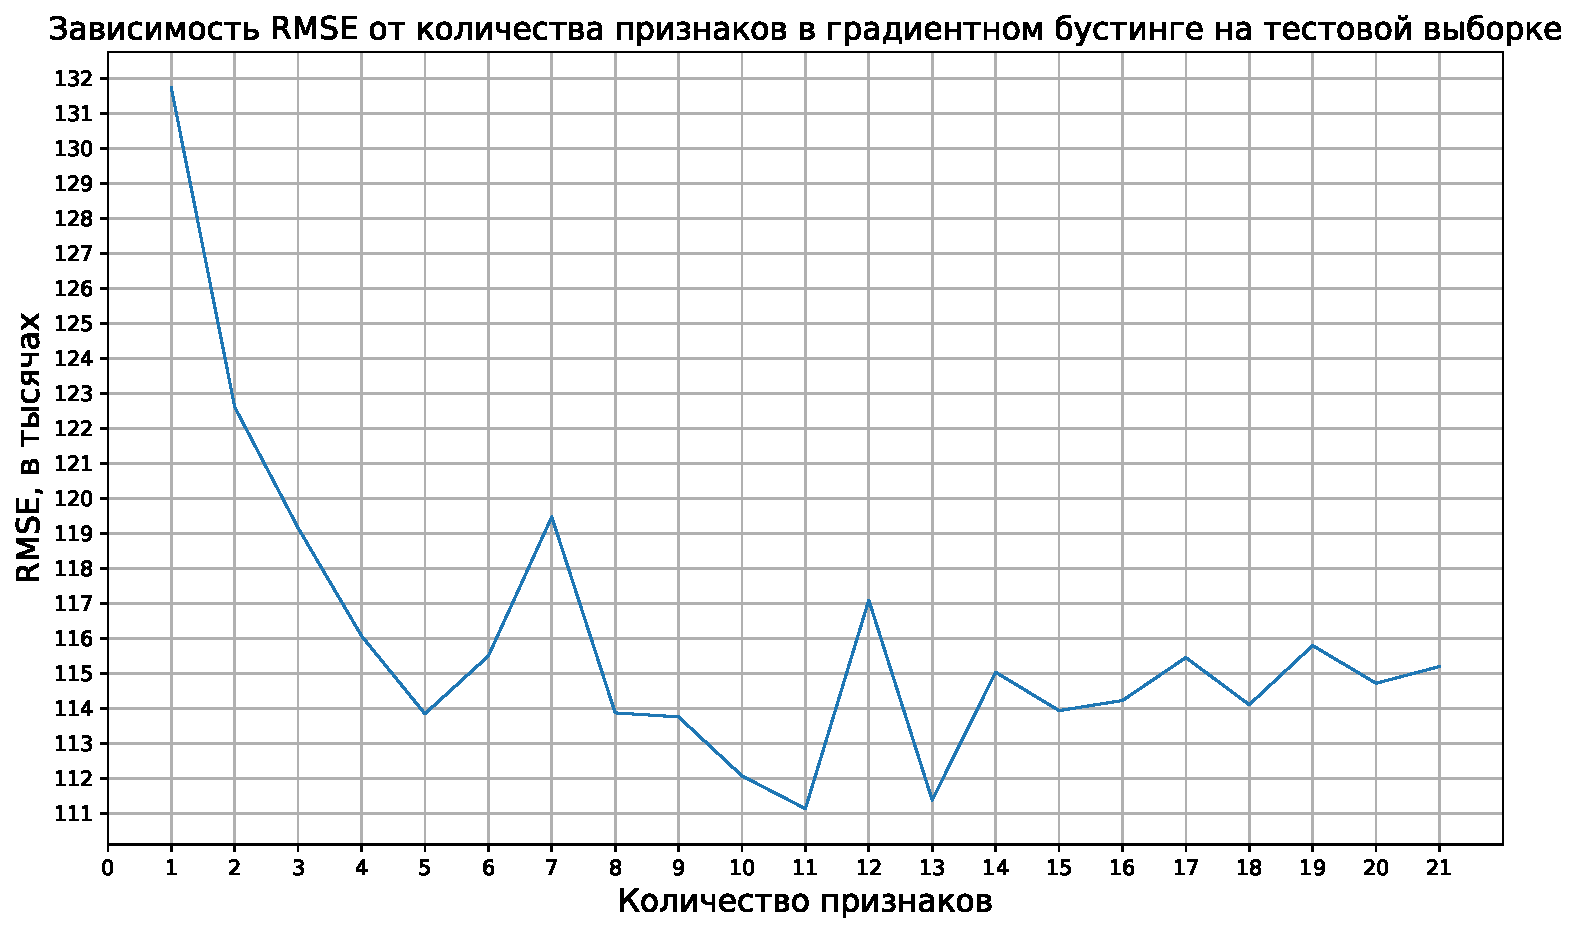
\includegraphics[scale=0.55]{5.1}}
\caption{Зависимость функции потерь (RMSE) от количества признаков}
\label{fig:image6}
\end{figure}
\subsection {Подбор оптимального количества признаков}
	Затем подбирается оптимальное количество признаков. Количество деревьев берется из предыдущего пункта, остальные параметры по умолчанию. Как видно из графика, оптимальным является среднее количество признаков, что отличает бустинг от случайного леса. При большом или слишком маленьком количестве признаков значение RMSE больше, чем у средних. 11 признаков можно принять оптимальным.

	По результатам экспериментов можно увидеть, что зависимость времени выполнения от количества признаков линейна.
\begin{figure}[h!]
\center{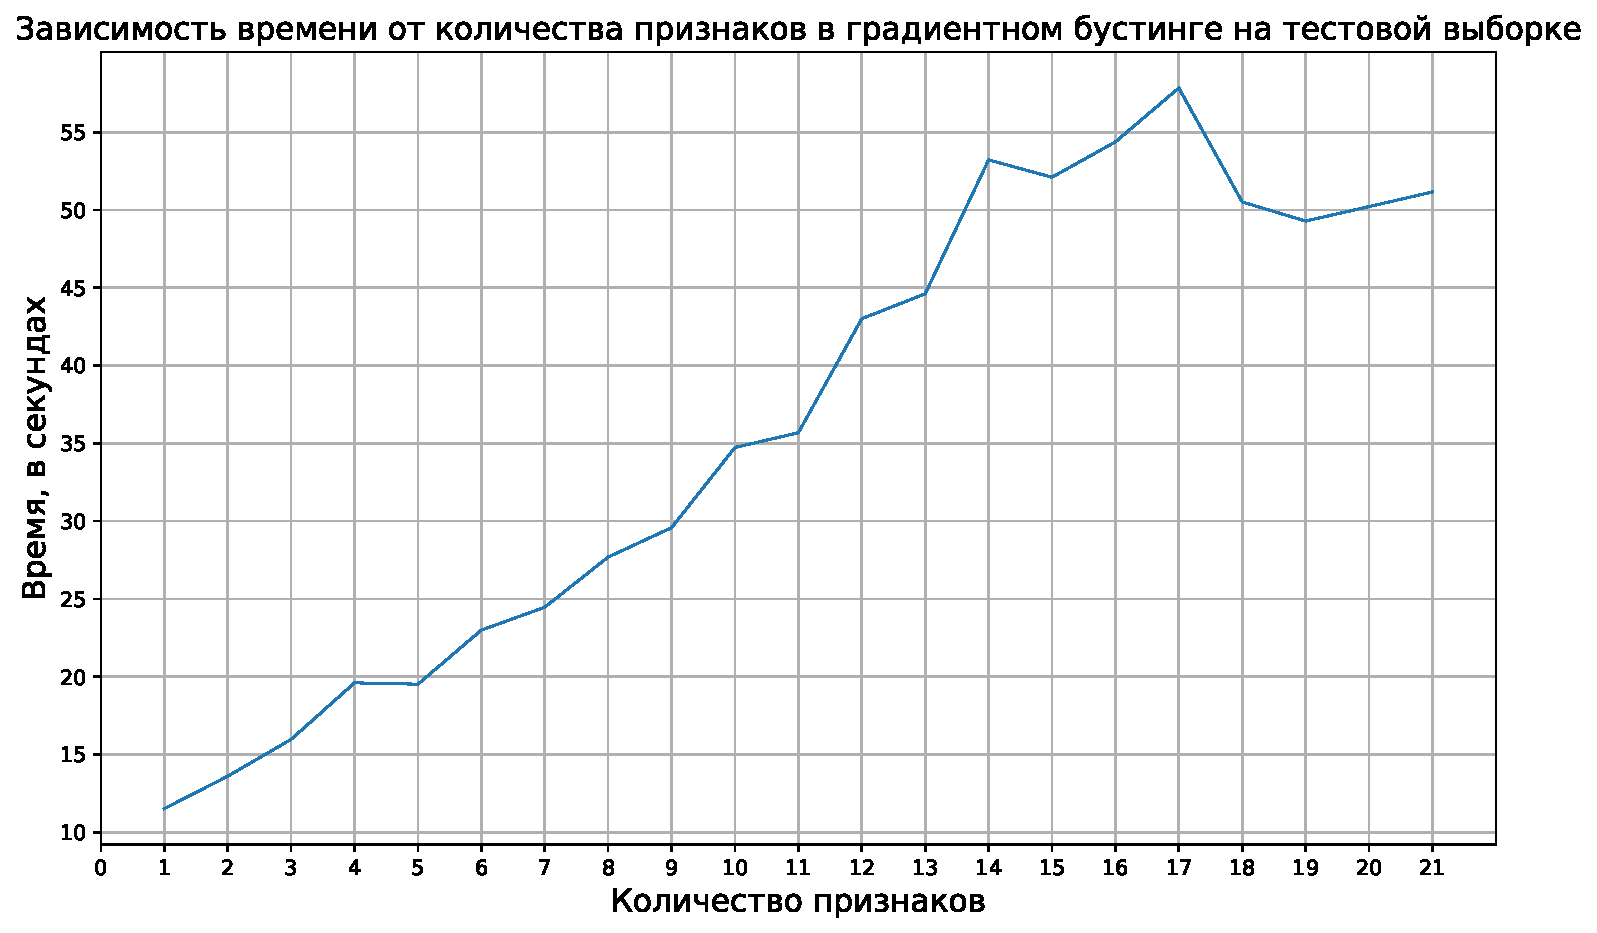
\includegraphics[scale=0.55]{5.2}}
\caption{Зависимость времени выполнения программы от количества признаков}
\label{fig:image6}
\end{figure}
\begin{figure}[h!]
\center{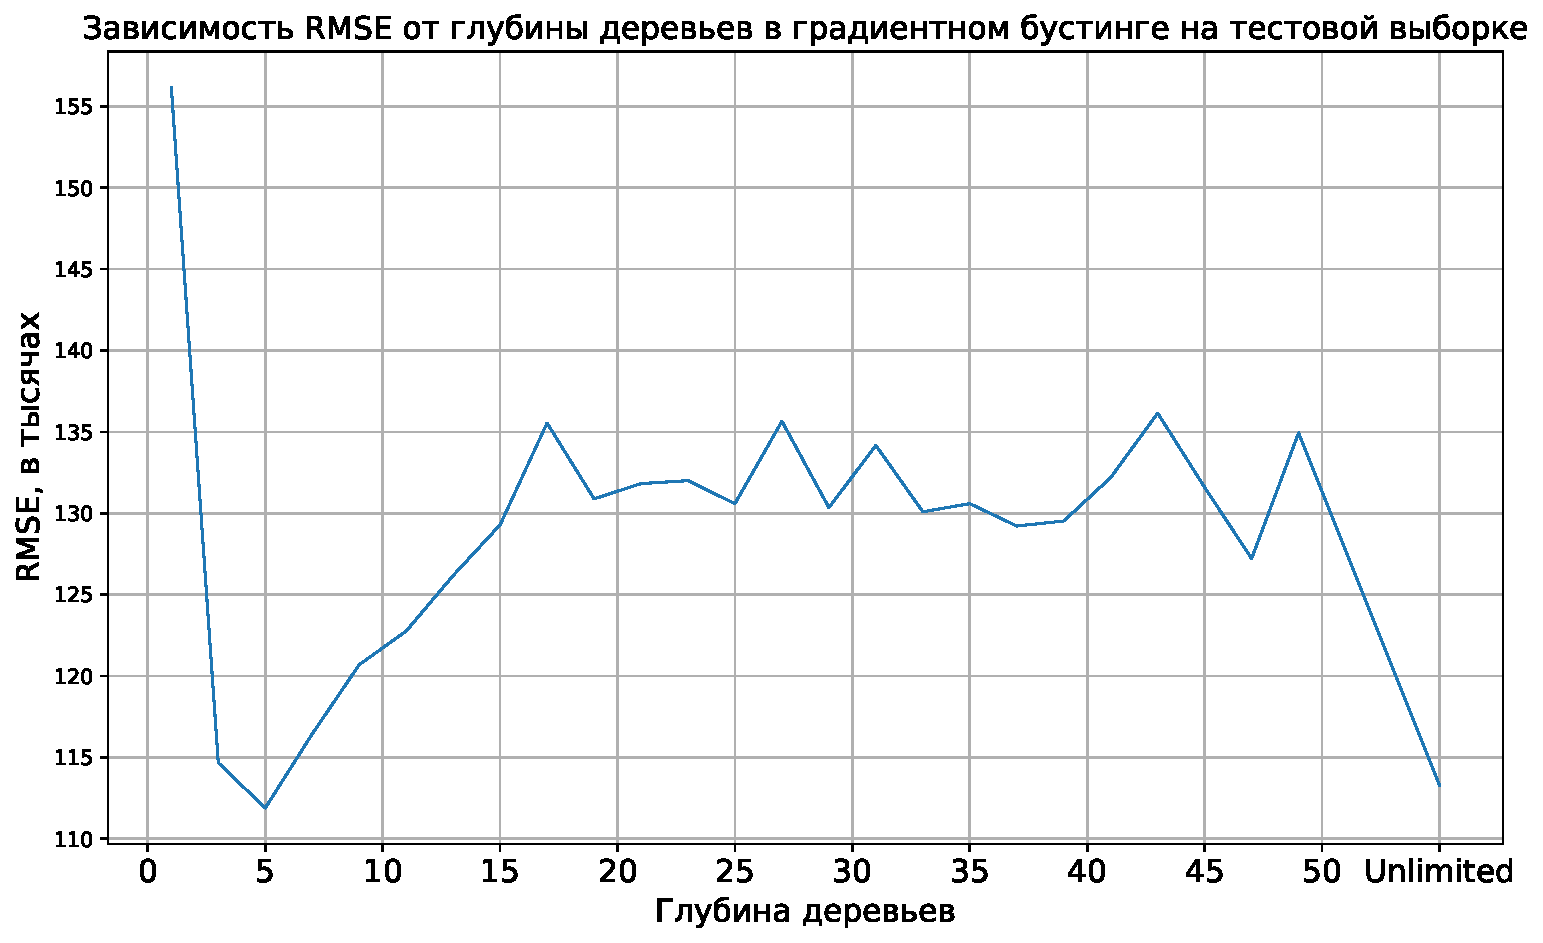
\includegraphics[scale=0.55]{6.1}}
\caption{Зависимость функции потерь (RMSE) от максимальной глубины деревьев}
\label{fig:image6}
\end{figure}
\subsection {Подбор оптимальной глубины деревьев}
	Подбирается оптимальное значение глубины деревьев. Количество деревьев и количество признаков берутся из предыдущих экспериментов, остальное по умолчанию. Тут алгоритм вновь отличается от случайного леса: вместо ансамблей с глубокими деревьями оптимальными стали ансамбли с малой максимальной глубиной. То есть переобученные деревья будут давать худший результат.

	Время работы алгоритма линейно при небольших значениях глубины, а затем становится почти постоянным. Оптимальным берется значение глубины равное 5.

\begin{figure}[h!]
\center{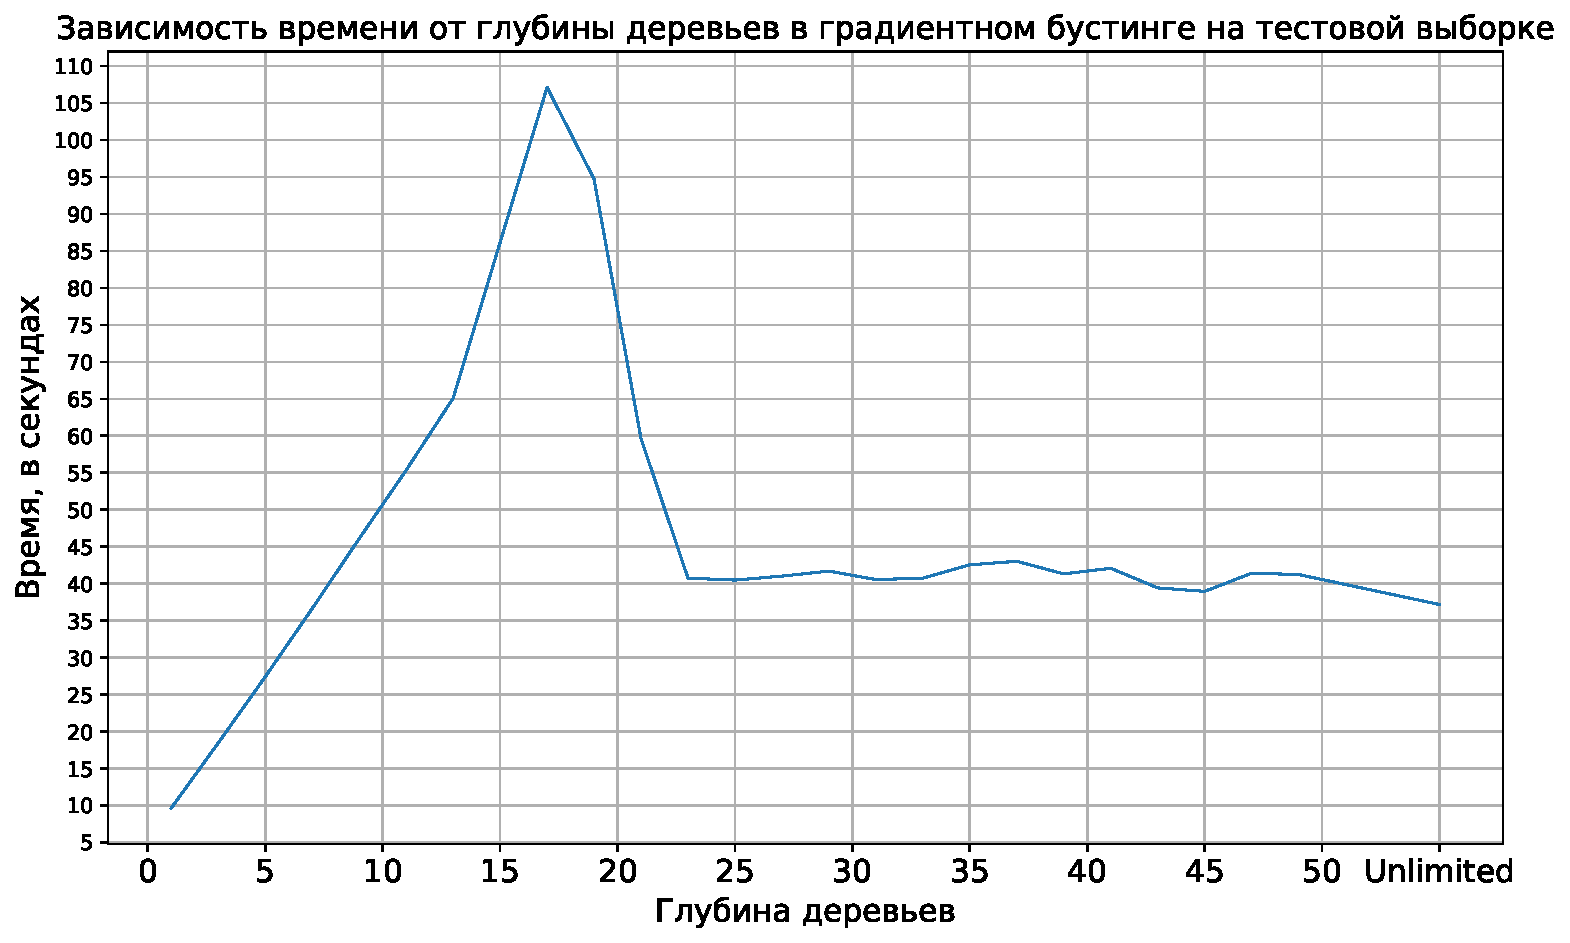
\includegraphics[scale=0.55]{6.2}}
\caption{Зависимость времени выполнения программы от максимальной глубины деревьев}
\label{fig:image6}
\end{figure}
\begin{figure}[h!]
\center{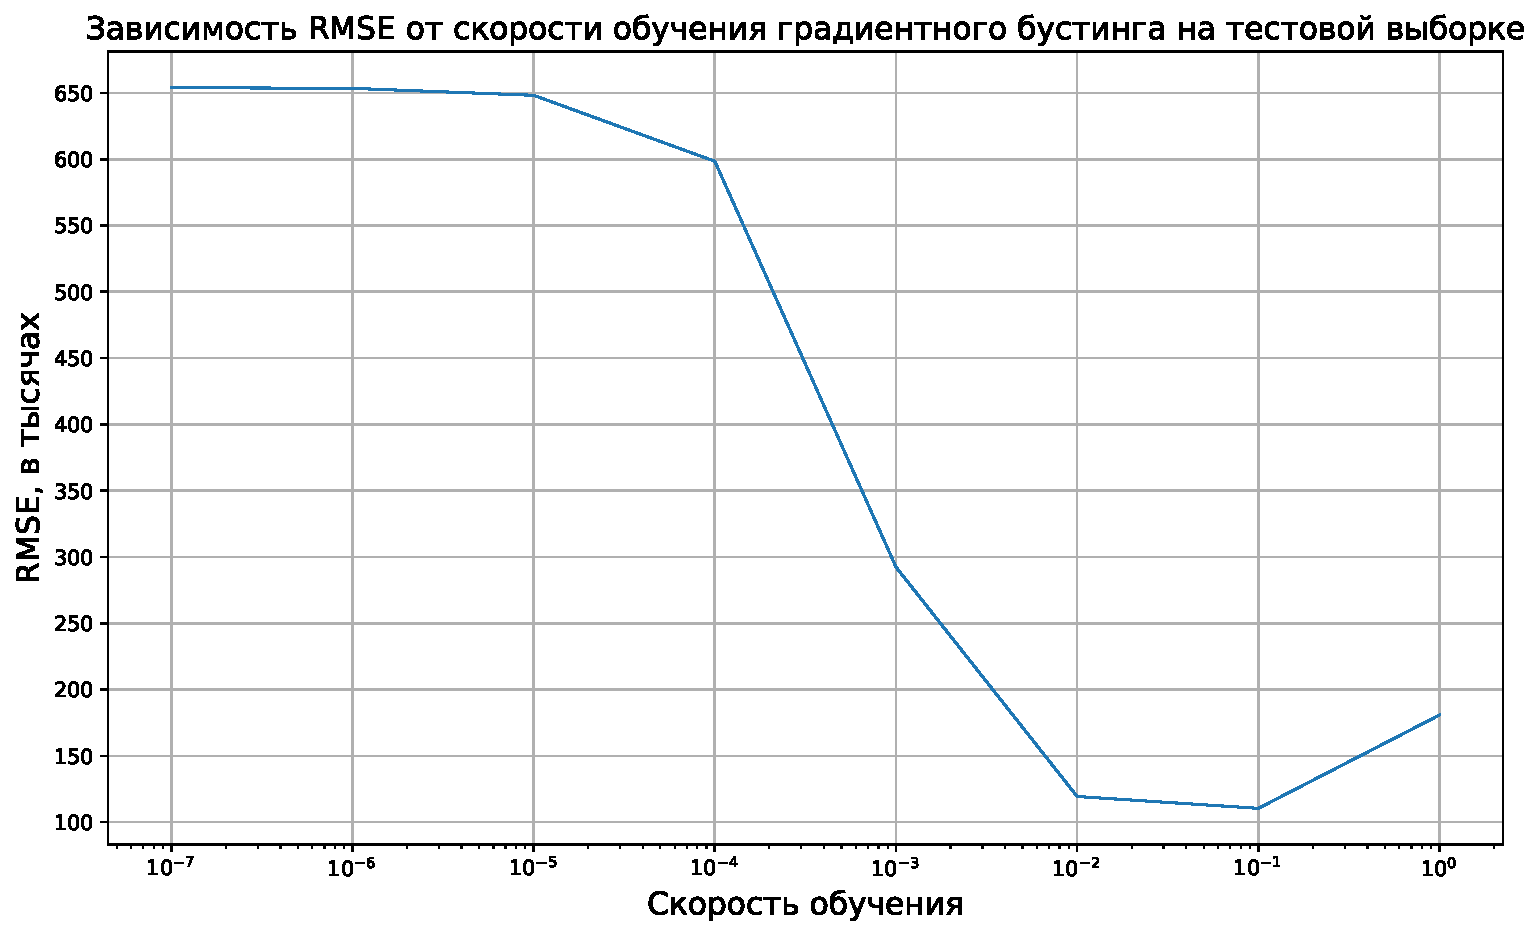
\includegraphics[scale=0.55]{7.1}}
\caption{Зависимость функции потерь (RMSE) от скорости обучения}
\label{fig:image7}
\end{figure}
\subsection {Подбор оптимального значения скорости обучения}
	В данном эксперименте подбирается оптимальное значение скорости обучения. Как видно, при малых значениях параметра модель недообучается, а при значениях близких к 1 переобучается. Поэтому можно считать оптимальным значение в 0.1.

	Время работы алгоритма не зависит от данного параметра, что можно заметить по графику. Результаты отличаются незначительно.

\begin{figure}[h!]
\center{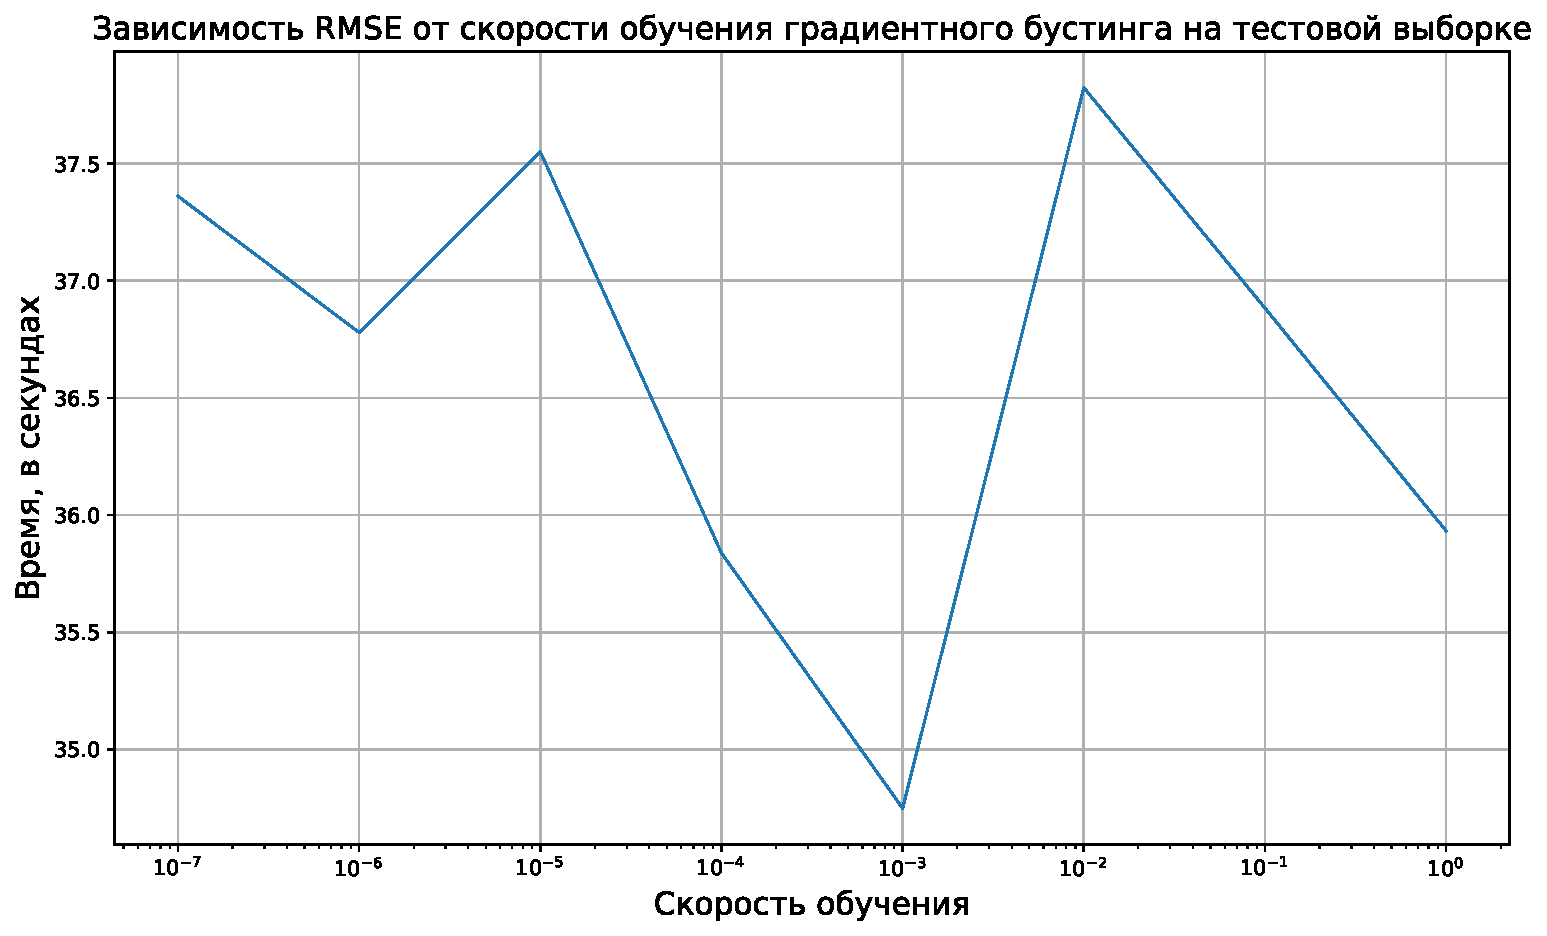
\includegraphics[scale=0.55]{7.2}}
\caption{Зависимость времени выполнения программы от скорости обучения}
\label{fig:image8}
\end{figure}

\section {Выводы}
Было проведено исследование случайного леса и градиентного бустинга. Были выяснены оптимальные параметры для каждого из алгоритмов. На представленных данных случайный лес оказался лучше градиентного бустинга (у случайного леса RMSE < 120, а у градиентного бустинга >120). 
\end{document}